\documentclass[a4paper]{article}
\usepackage[spanish]{babel}
\usepackage[pdftex,usenames,dvipsnames]{color}
\usepackage{multicol}
\usepackage{graphicx}
\usepackage{listings}
\usepackage{color}
\usepackage{hyperref}
\usepackage{vmargin}

\definecolor{dkgreen}{rgb}{0,0.6,0}
\definecolor{gray}{rgb}{0.5,0.5,0.5}
\definecolor{mauve}{rgb}{0.58,0,0.82}

\lstset{
    language=bash, 
    basicstyle=\footnotesize\color{black},
    backgroundcolor=\color{white},
    morekeywords={durar@durar, restart}, keywordstyle=\color{green},
    classoffset=1,
    showspaces=false,
    showstringspaces=false,
    showtabs=false,
    frame=single, 
    tabsize=2,
    captionpos=b,
    breaklines=true,
}
\lstdefinestyle{bashCentOS}{
    language=bash, 
    basicstyle=\footnotesize\color{black},
    backgroundcolor=\color{white},
    morekeywords={durar@localhost, start}, keywordstyle=\color{red},
    classoffset=1,
    showspaces=false,
    showstringspaces=false,
    showtabs=false,
    frame=single, 
    tabsize=2,
    captionpos=b,
    breaklines=true,
}
\begin{document}
\pagestyle{plain}
\title{Práctica 4: Benchmarking y Ajuste del Sistema" \\ 
Ingeniería de Servidores}
\author{Raúl Durán Racero}
\begin{figure}
    \centering
    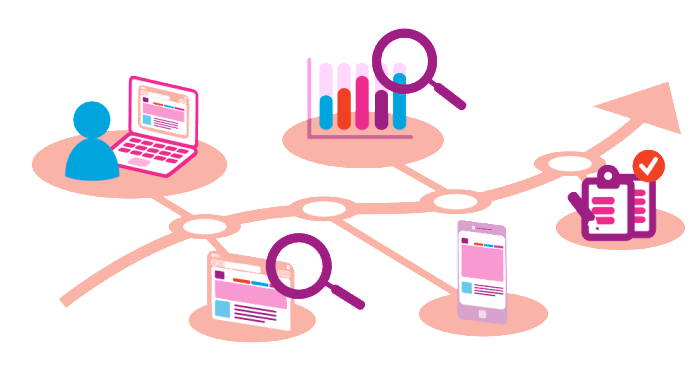
\includegraphics[width=\textwidth]{benchmarking004.png}
\end{figure}
\maketitle
\begin{figure}
    \centering
    \includegraphics[width=0.25\textwidth]{logoEtsiit.pdf}
\end{figure}

\newpage
\tableofcontents
\newpage
\section{Ejercicio 1}
Una vez que haya indagado sobre los \textsl{benchmarks} disponibles, seleccione 
como mínimo dos de ellos y proceda a ejecutarlos en \textbf{Ubuntu} y \textbf{CentOS}.
Comente las diferencias.
\subsection{Phoronix en UbuntuServer}
Lo primero que haremos será obtener el paquete de la página de Phoronix e instalarlo:
\begin{lstlisting}
    durar@durar:~$ sudo wget http://phoronix-test-suite.com/releases/repo/pts.debian/files/phoronix-test-suite_10.6.1_all.deb
    durar@durar:~$ sudo dpkg -i phoronix-test-suite_10.6.1_all.deb
\end{lstlisting}
Una vez instalado, podemos ver los diferentes tests y suites que dispone Phoronix:
\begin{lstlisting}
    durar@durar:~$ phoronix-test-suite list-available-tests
    durar@durar:~$ phoronix-test-suite list-available-suites
\end{lstlisting}
De la lista de tests, escogeremos dos. En mi caso, he escogido los siguientes:
\subsection*{\textbf{pts/sudokut:}}
Sudokut es un test que mide cuánto tiempo tarda el sistema en resolver 100 puzzles 
\textsl{Sudoku} escritos en TCL (\textsl{Tool Command Language}):
\begin{lstlisting}
    durar@durar:~$ phoronix-test-suite benchmark pts/sudokut 
\end{lstlisting}
\subsection*{\textbf{pts/ramspeed:}}
RAMspeed SMP comprueba como actúa la RAM de nuestro sistema:
\begin{lstlisting}
    durar@durar:~$ phoronix-test-suite benchmark pts/ramspeed 
\end{lstlisting}
Nos pedirá que escojamos distintas ocpiones. Escogemos las que queramos (en mi caso, 
solo compararé la función \textsl{Add}):

Si hay errores a la hora de instalar las dependencias necesarias para los tests, 
intenta actualizar:
\begin{lstlisting}
    durar@durar:~$ sudo apt-get update
\end{lstlisting}

\subsection{Phoronix en CentOS}
Repetimos los pasos de instalación que hicimos en UbuntuServer (si tienes instalados
en CentOS wget y dpkg):
\begin{lstlisting}[style=bashCentOS]
    [durar@localhost ~]$ sudo wget http://phoronix-test-suite.com/releases/repo/pts.debian/files/phoronix-test-suite_10.6.1_all.deb
    [durar@localhost ~]$ sudo dpkg -i phoronix-test-suite_10.6.1_all.deb
\end{lstlisting}
Y volvemos a comrpobar los tests y suites:
\begin{lstlisting}[style=bashCentOS]
    [durar@localhost ~]$ phoronix-test-suite list-available-tests
    [durar@localhost ~]$ phoronix-test-suite list-available-suites
\end{lstlisting}
Ejecutaremos los mismos tests que en UbuntuServer para comparar resultados:
\begin{lstlisting}[style=bashCentOS]
    [durar@localhost ~]$ phoronix-test-suite benchmark pts/sudokut
    [durar@localhost ~]$ phoronix-test-suite benchmark pts/ramspeed
\end{lstlisting}

\subsection{Comparación de Resultados}
\subsection*{\textbf{Sudokut:}}
\begin{figure}[hbt!]
    \centering
    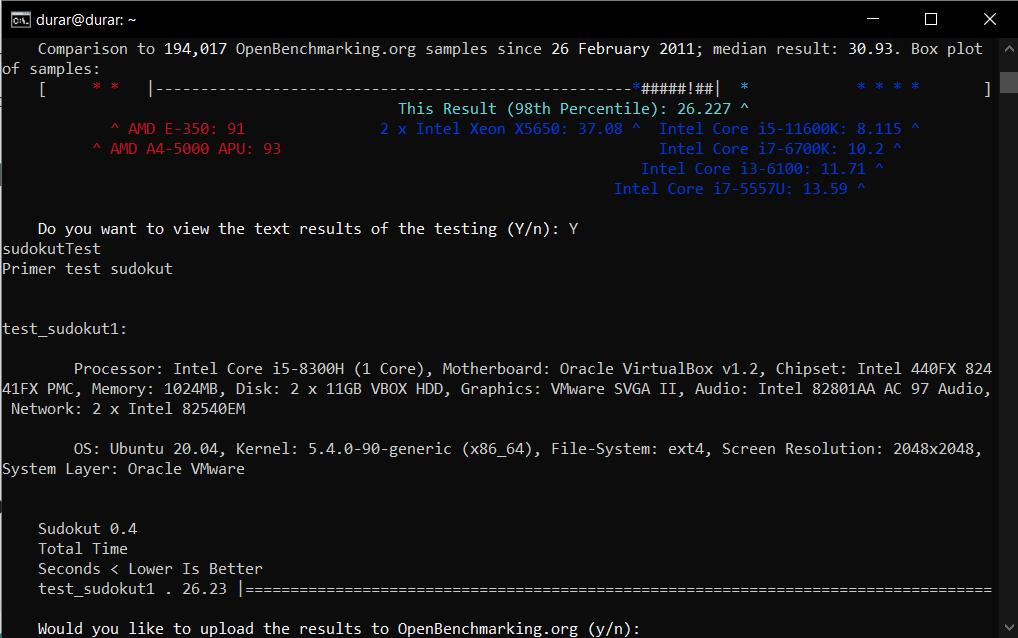
\includegraphics[width=\textwidth]{resultado_sudokut1.png}
    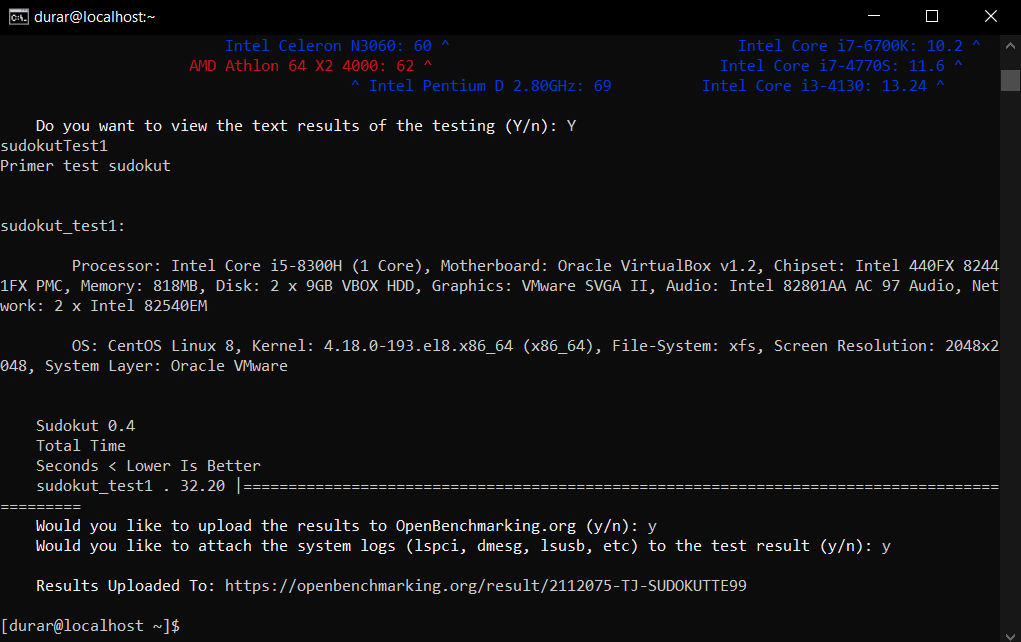
\includegraphics[width=\textwidth]{resultado_sudokut_centos.png}
\end{figure}
Podemos ver como en la primera imagen (UbuntuServer), el test Sudokut ha tardado menos 
en ejecutarse (26.23s) que en CentOS (32.29s).
\subsection*{\textbf{RAMspeed:}}
\newpage
\begin{figure}[hbt!]
    \centering
    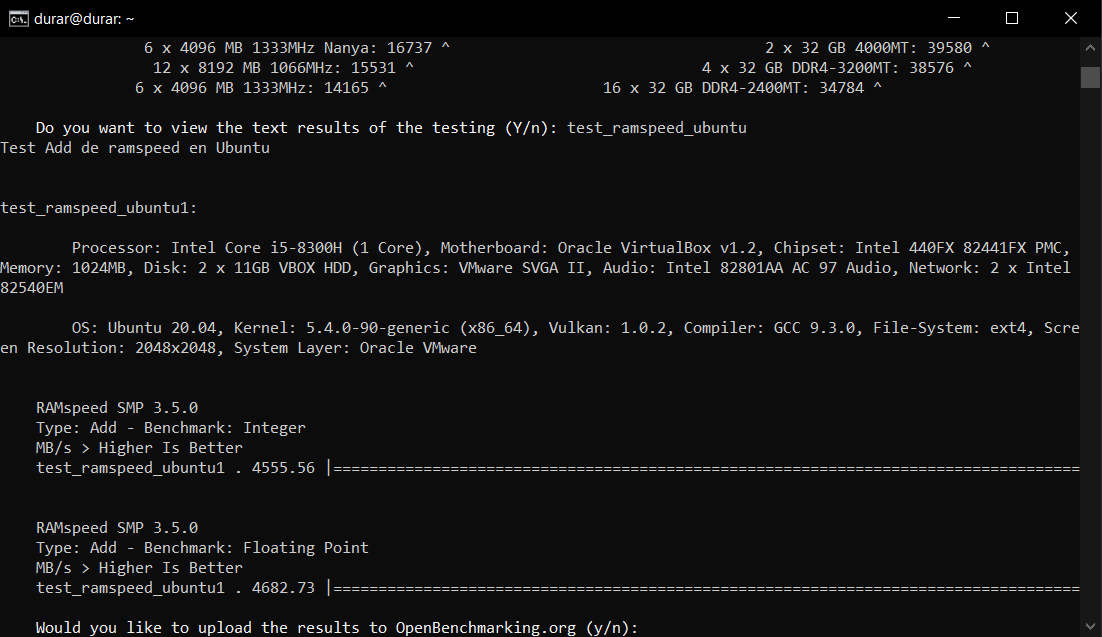
\includegraphics[width=\textwidth]{resultado ramspeed ubuntu.png}
    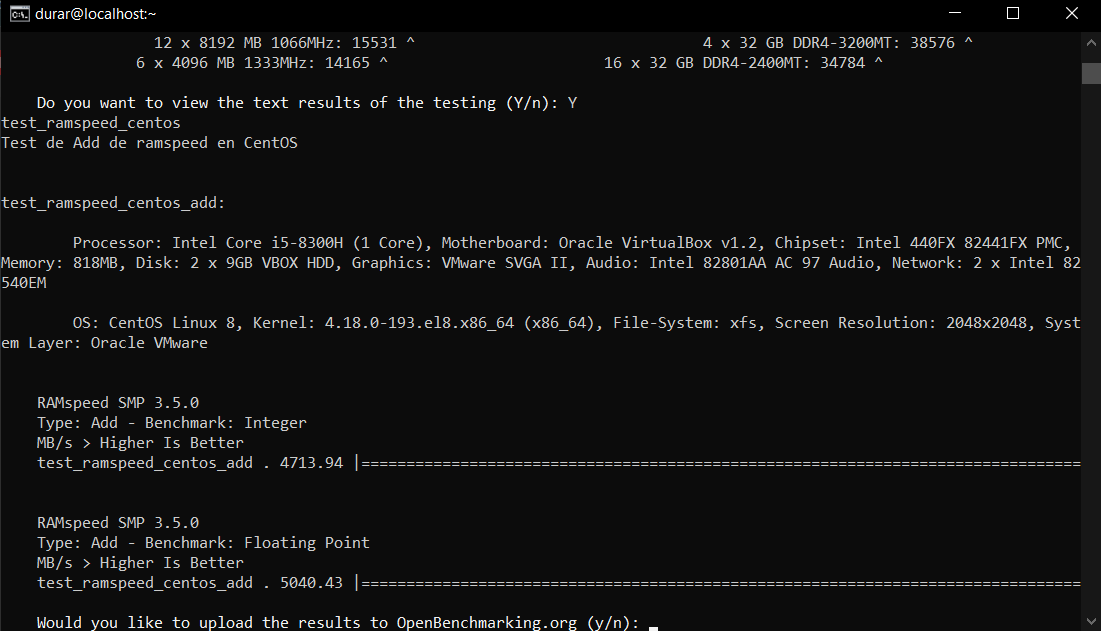
\includegraphics[width=\textwidth]{resultado ramspeed centos.png}
\end{figure}
Vemos que los resultados obtenidos en CentOS son mejores que en Ubuntu. Además, en ambos sistemas
el resultado de Add con variables enteras son peores que con coma flotante.
\newpage
\section{Ejercicio 2}
Tras probar un test básico para una web, utilizaremos Jmeter para hacer 
un test sobre una aplicación que ejecuta sobre dos contenedores (uno
para la BD y otro para la aplicación en sí). El código está disponible en 
\href{https://github.com/davidPalomar-ugr/iseP4JMeter}{https://github.com/davidPalomar-ugr/iseP4JMeter}
donde se dan detalles sobre cómo ejecutar la aplicación en una de nuestras máquinas virtuales.

El servidor se distribuye en forma de  una aplicación de contenedores Docker sobre
Compose, por lo que necesitaremos ambas aplicaciones:
\begin{lstlisting}
    durar@durar:~$ sudo apt-get install docker docker-compose
\end{lstlisting}
Ahora clonaremos el repositorio de \href{https://github.com/davidPalomar-ugr/iseP4JMeter}{https://github.com/davidPalomar-ugr/iseP4JMeter}:
\begin{lstlisting}
    durar@durar:~$ git clone https://github.com/davidPalomar-ugr/iseP4JMeter
\end{lstlisting}
Una vez lo hemos descargado, nos situamos al nivel del archivo docker-compose.yml y ejecutamos:
\begin{lstlisting}
    durar@durar:~/iseP4JMeter$ sudo docker-compose up
    durar@durar:~/iseP4JMeter$ sudo docker-compose down
\end{lstlisting}
Con esto, Docker descargará las imágenes base y construirá las nuevas imágenes para
la aplicación. 
Podemos comprobar que funciona el servicio correctamente buscando en nuestro navegador:
\textbf{IP:3000}. Primero deberemos de abrir el puerto 3000 e instalar en UbuntuServer
mongodb, ya que este sistema de base de datos es necesario para que funcione nuestro servicio. 
Tendremos esta interfaz: \newline
\begin{figure}[hbt!]
    \centering
    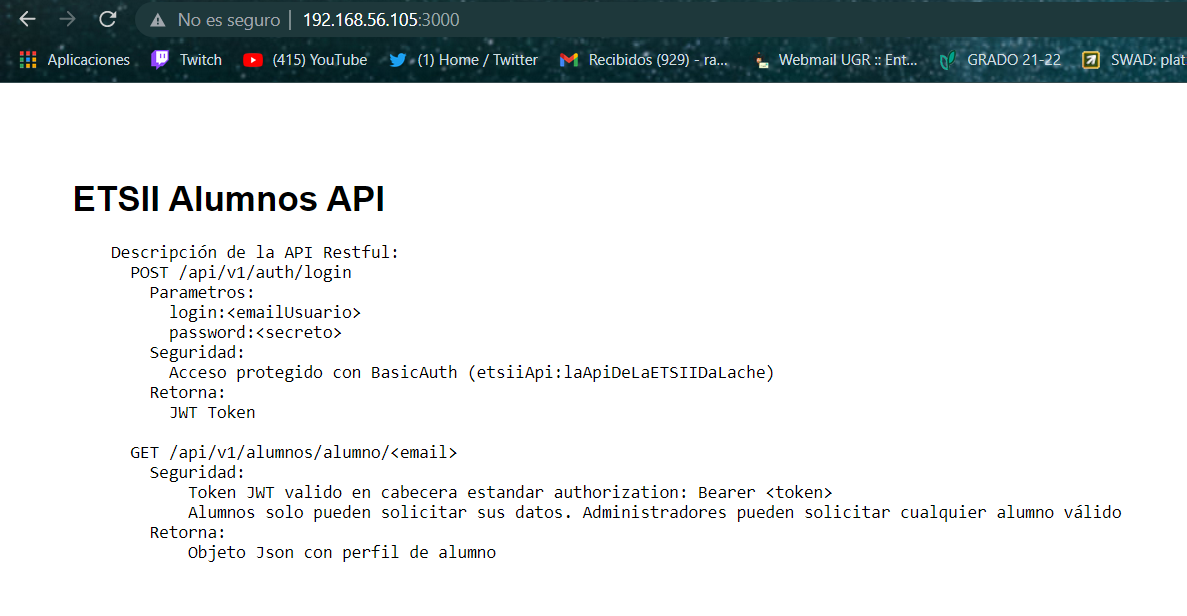
\includegraphics[width=\textwidth]{direccion docker.png}
\end{figure}
\newpage
Ahora, tenemos que instalar \textbf{JMeter} en nuestro sistema host.
Descargamos el paquete de JMeter y abrimos el ejecutable \textsl{ApacheJMeter} de la carpeta \textsl{bin} del 
archivo comprimido. Es necesario tener una versión de \textbf{Java 8} o superior.
\begin{figure}[hbt!]
    \centering
    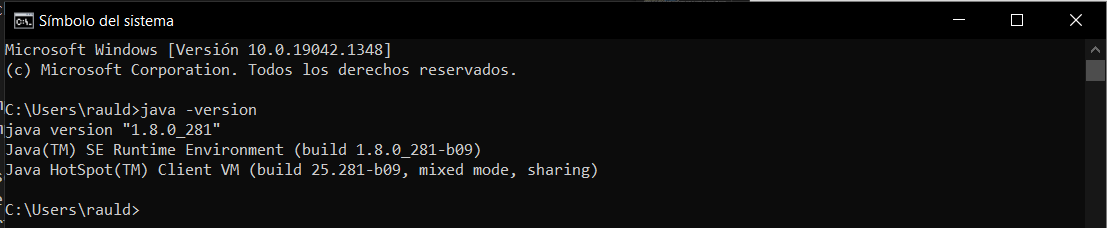
\includegraphics[width=\textwidth]{version java.png}
\end{figure}
\newline Tendremos una interfaz como esta:
\begin{figure}[hbt!]
    \centering
    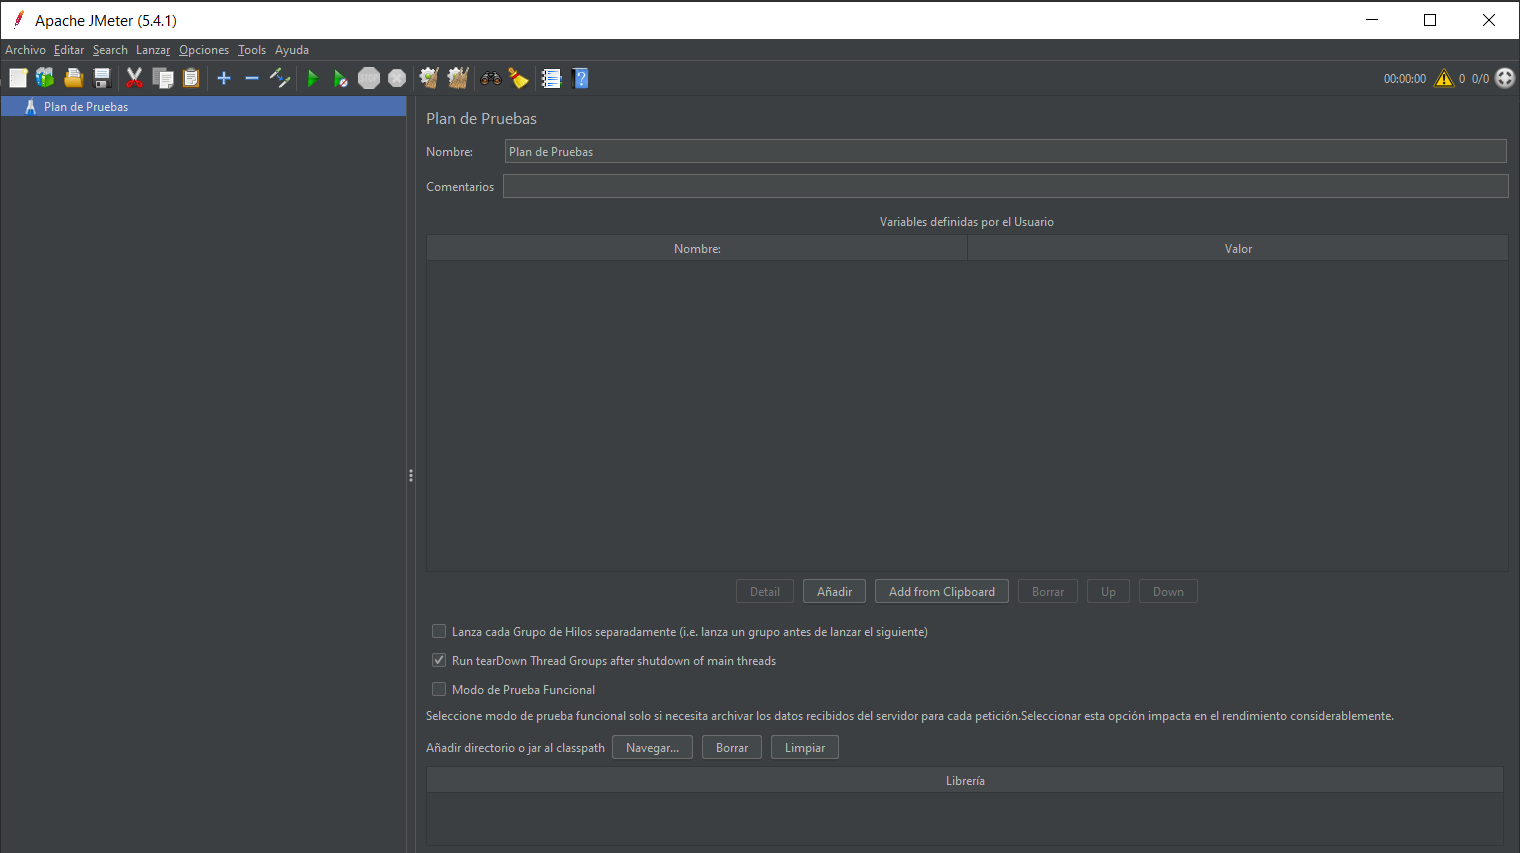
\includegraphics[width=\textwidth]{interfaz apache jmeter.png}
\end{figure}
\newpage
\subsection{Test debe tener parametrizados el Host y el Puerto en el Test Plan}
\begin{figure}[hbt!]
    \centering
    \includegraphics[width=\textwidth]{añadir host y port.png}
\end{figure}
\subsection{Hacer 2 grupos de hebras distintos para simular al acceso de los alumnos
y los administradores}
Se nos dice que los credenciales de alumno y administrador se cogen de los archivos
\textsl{alumnos.csv} y \textsl{administrador.csv}, respectivamente, que se encuentran en
el directorio iseP4JMeter/jMeter. Antes de hacer esto, escogeremos un 
administrador y un alumno (hacemos cat de los archivos .csv), para simplificar
la comprobación del resto de pasos. Cogeremos los credenciales desde estos
archivos como último paso. Yo he escogido:
\begin{description}
    \item[Administrador, contraseña:] suarezgraves@etsii.ugr.es, laborum
    \item[Alumno, constraseña:] margretdonovan@tropoli.com, non  
\end{description}
Ya escogidos nuestro administradory nuestro alumno, creamos 2 grupos de hebras 
en JMeter, uno para el administrador y el otro para el alumno. Para ello:
\begin{figure}[hbt!]
    \centering
    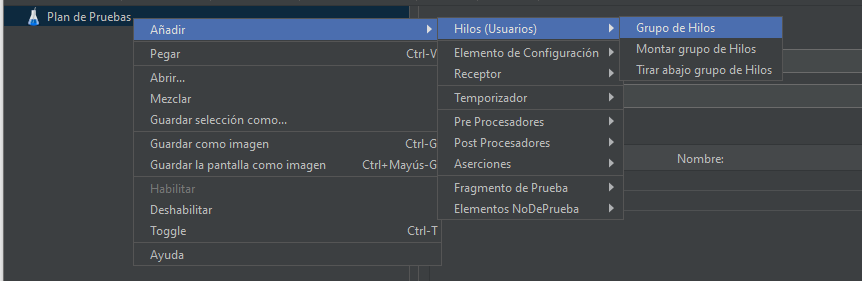
\includegraphics[width=\textwidth]{crear grupo hilos.png}
\end{figure}
Dejamos la configuración por defecto. \newline
Ahora, añadimos una petición por defecto HTTP:
\newpage
\begin{figure}[hbt!]
    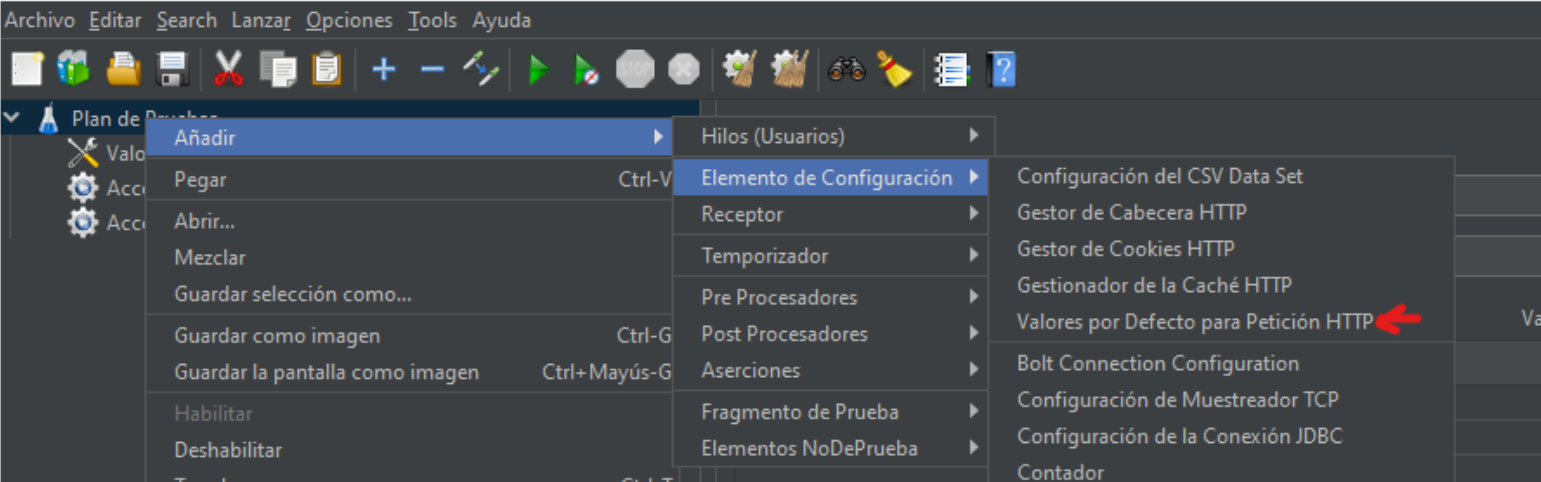
\includegraphics[width=\textwidth]{valores por defecto peticion.png}
\end{figure}
Y metemos nuestros parámetros Host y Port (se escribe de la forma \$\{param\}):
\begin{figure}[hbt!]
    \includegraphics[width=\textwidth]{añadir param host y port.png}
\end{figure}
\newline Esto lo hemos hecho para no tener que repetir Host y Port en cada petición.
Para simular el acceso de un administrador y un alumno, creamos una petición HTTP para
cada grupo de hebra, donde tendremos que introducir la ruta, usuario, constraseña, y tipo de peticion:
\begin{figure}[hbt!]
    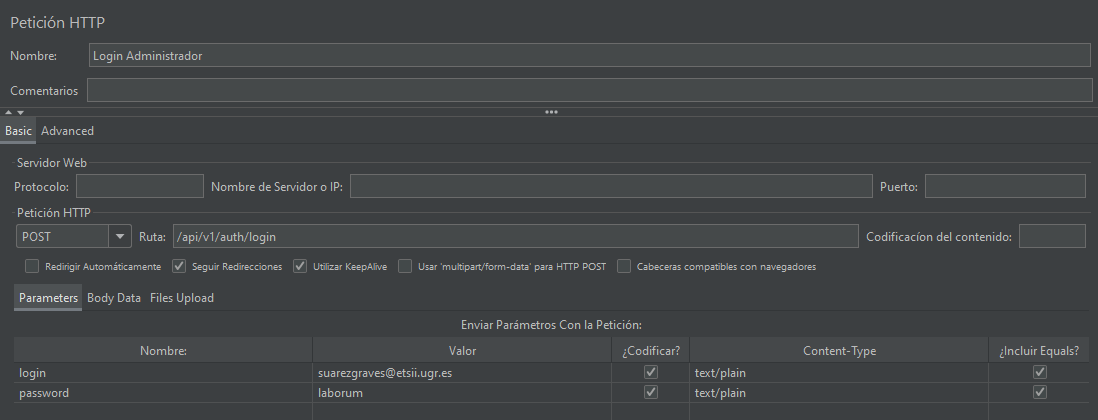
\includegraphics[width=\textwidth]{login administrador.png}
    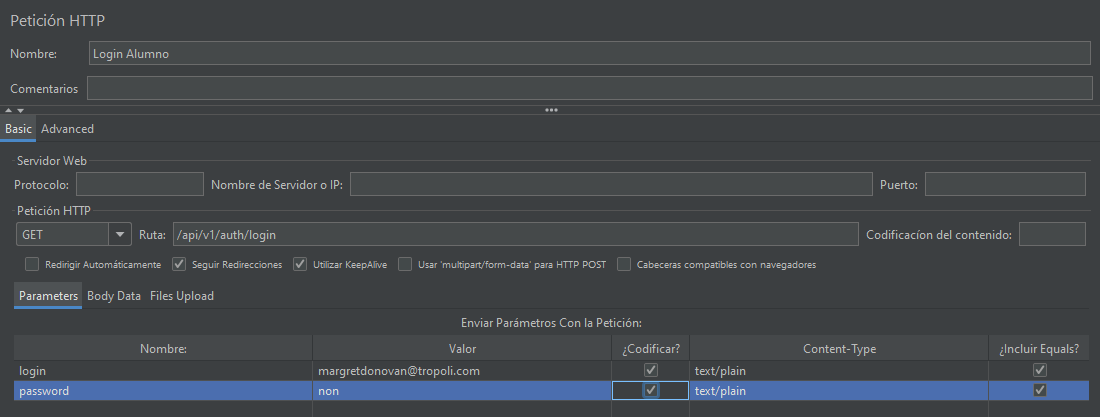
\includegraphics[width=\textwidth]{login alumno.png}
\end{figure}
\newpage
La ruta la podemos encontrar en el script pruebaEntorno.sh.
Para ver el resultado de los accesos, podemos usar un árbol de resultados para ambos
grupos de hilos:
\begin{figure}[hbt!]
    \includegraphics[width=\textwidth]{añadir arbol resultados.png}
\end{figure}
\newline Al ejecutarlo, veremos que nos da el mismo error para ambos accesos, indicando 
que no está autorizado:
\begin{figure}[hbt!]
    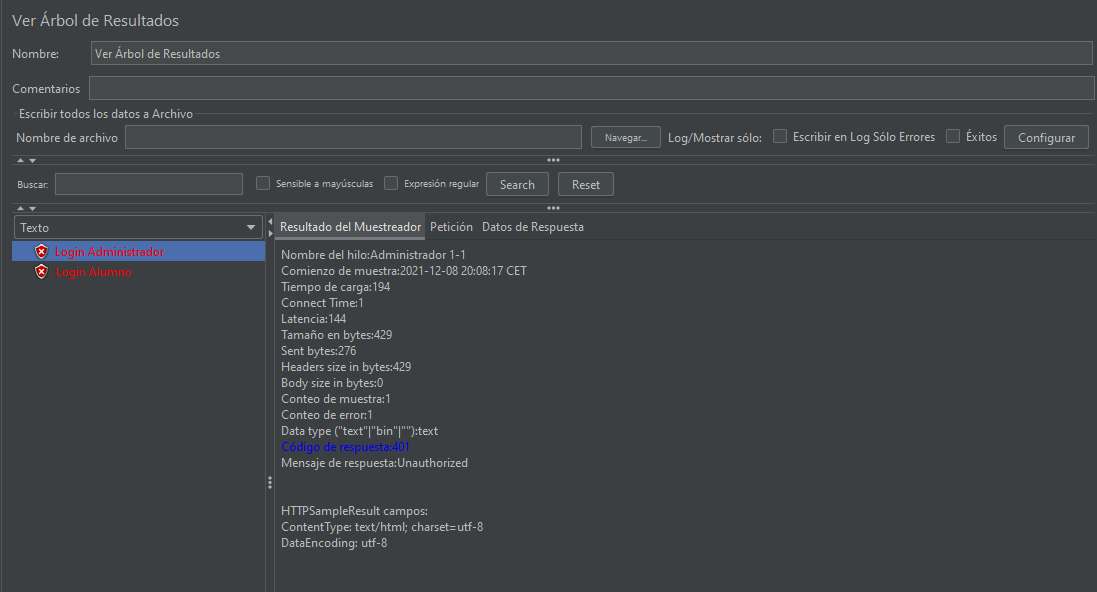
\includegraphics[width=\textwidth]{errores arbol resultados.png}
\end{figure}
\newpage Esto se debe a que nos falta el gestor de autorización HTTP para 
cada grupo de hebras, ya que el acceso al servicio está protegido por HTTP BasicAuth:
\begin{figure}[hbt!]
    \includegraphics[width=\textwidth]{añadir gestor autorizacion.png}
\end{figure}
\newline Lo configuramos: 
\begin{figure}[hbt!]
    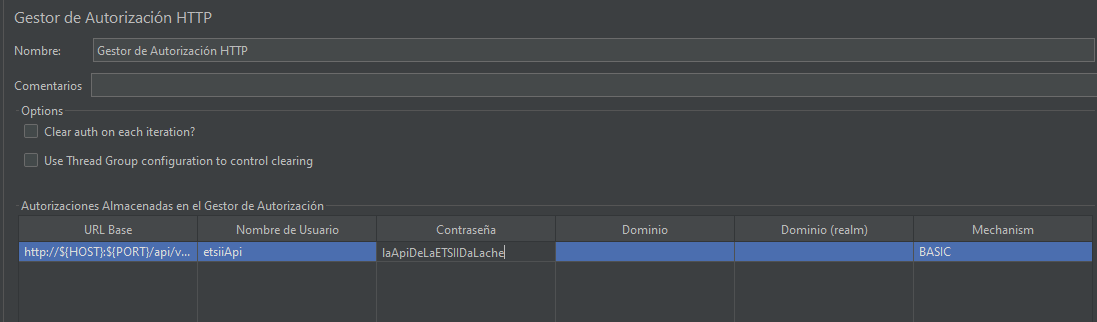
\includegraphics[width=\textwidth]{gestor autorizacion configurado.png}
\end{figure}
\newline Podemos ver el nombre de usuario y la contraseña en el archivo mencionado anteriormente
pruebaEntorno.sh.
\newpage
Volvemos a arrancar JMeter, y esta vez habrán accedido correctamente:
\begin{figure}[hbt!]
    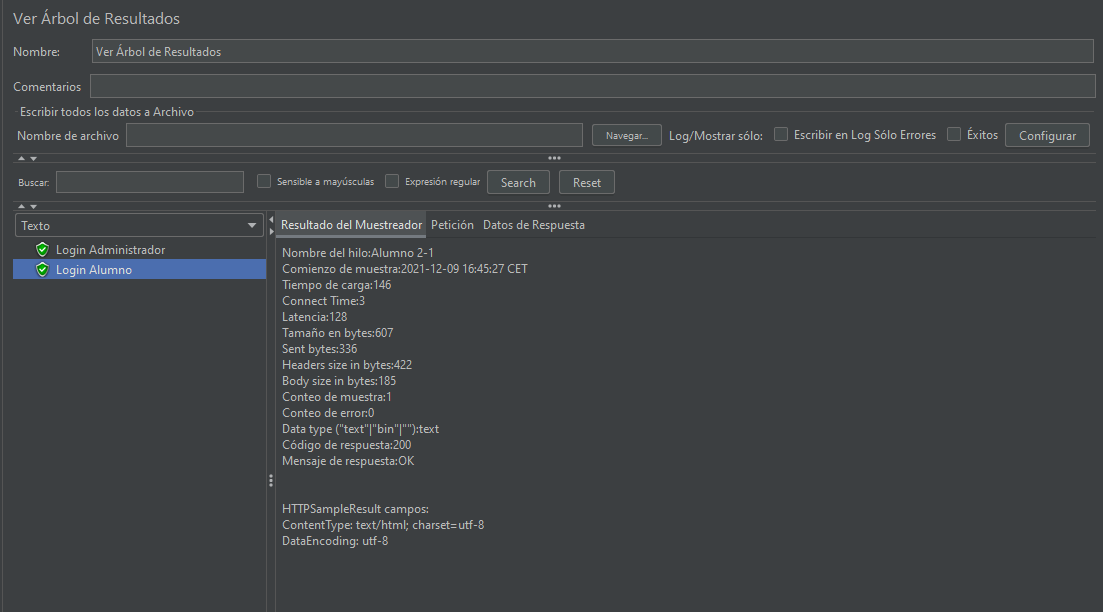
\includegraphics[width=\textwidth]{login alumno correcto.png}
    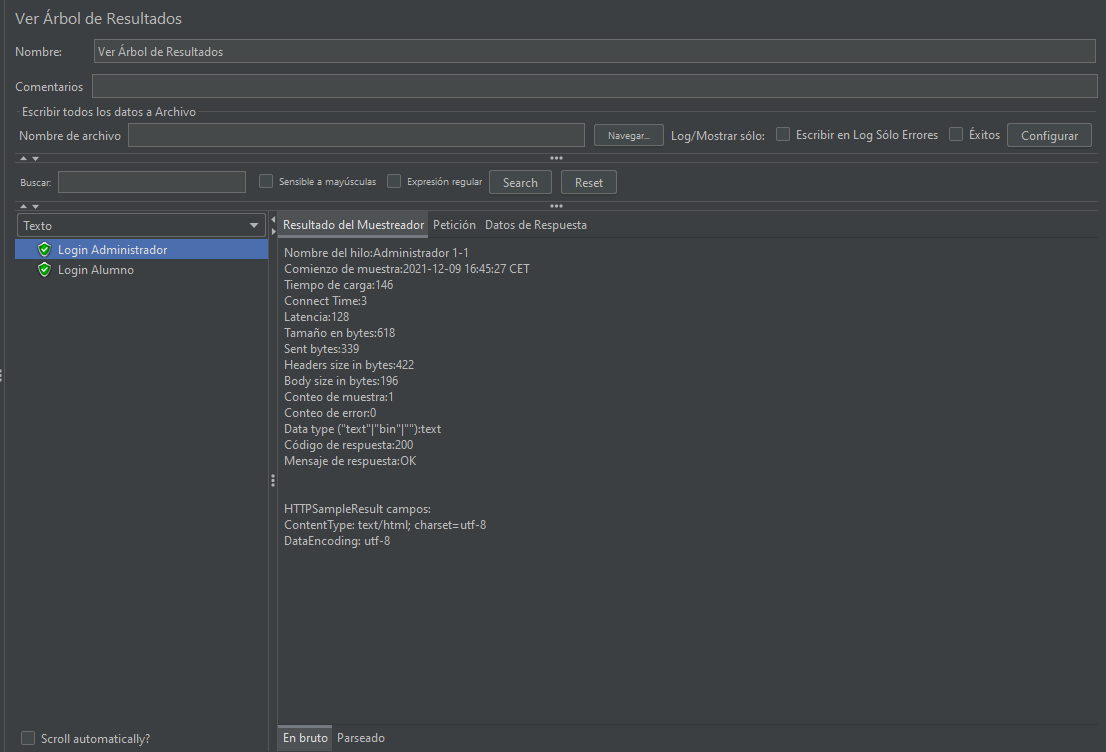
\includegraphics[width=\textwidth]{login administrador correcto.png}
\end{figure}
\newpage
\subsection{Añadimos esperas aleatorias (Gaussian Random Timer)}
\begin{figure}[hbt!]
    \centering
    \includegraphics[width=\textwidth]{añadir temporizadorg.png}
\end{figure}
\subsection{Recuperar datos alumno}
Tenemos que hacer una petición HTTP para recuperar los datos del alumno:
\begin{figure}[hbt!]
    \centering
    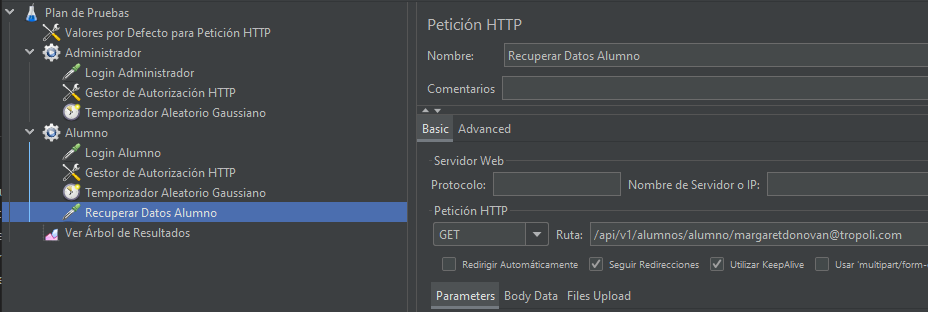
\includegraphics[width=\textwidth]{recuperar datos alumno.png}
\end{figure}
\newline La ruta la encontraremos, una vez más, en el pruebaEntorno.sh (al final del mismo).
Repetimos para el administrador (Acceso Administrador). En la ruta, deberemos poner 
el login de un administrador, ya que si usamos el de un alumno, nos dará error, ya que 
un alumno no puede consultar los datos de otro alumno.
\subsection{Muestreo recogido por apiAlumnos.log}
Se nos pide que el muestreo para simular el acceso de los administradores lo
debe coger el archivo apiAlumnos.log, usando un Muestreador de Acceso a Log:
\newpage
\begin{figure}
    \centering
    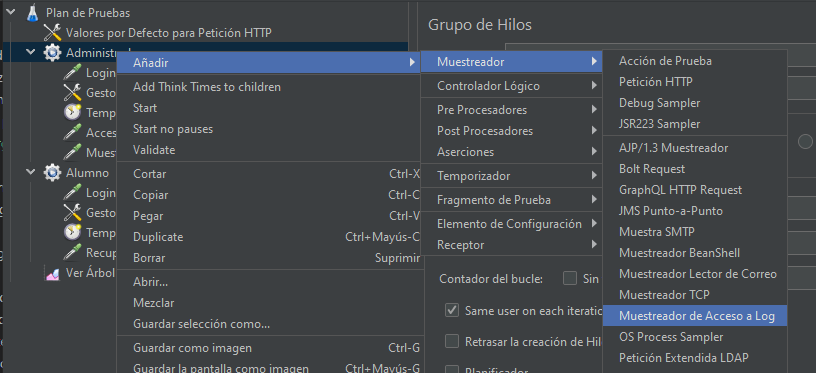
\includegraphics[width=\textwidth]{muestreador de acceso a log1.png}
    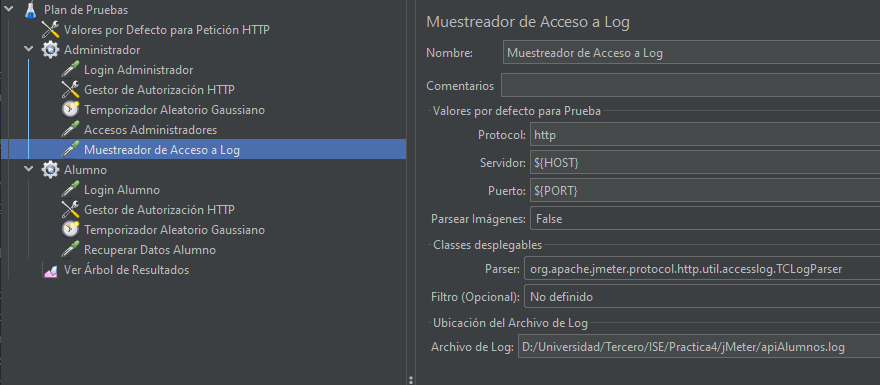
\includegraphics[width=\textwidth]{muestrador configurado1.png}
\end{figure}
\subsection{Usar expresión regular para extrar token JWT}
Tenemos que utilizar una expresión regular para poder extraer el token JWT que hay 
que añadir a la cabecera de las peticiones. Usaremos el Gestor de Cabecera HTTP:
\begin{figure}[hbt!]
    \centering
    \includegraphics[width=\textwidth]{añadir gestor cabecera http.png}
\end{figure}
\newpage
También tendremos que añadir un extractor de expresiones regulares para obtener el token:
\begin{figure}[hbt!]
    \centering
    \includegraphics[width=\textwidth]{añadir extractor de expr reg.png}
\end{figure}
\newline Tendremos varios apartados que debemos configurar:
\begin{description}
    \item[Nombre de referencia:] Nombre de la variable en la que se guardará el
    texto extraído. 
    \item[Expresión Regular:] El patrón con el que el texto hará 'match'. Usaremos los siguientes carácteres especiales:
    \begin{description}
        \item[.]  empareja cualquier caracter
        \item[+]  uno o más veces 
        \item[?]  para cuando encuentra el primer 'match' exitoso
    \end{description} 
    \item[Plantilla:] Agrupa los strings entre paréntesis. Con \$1\$ selecciona el primero.
    \item[Coincidencia No.:] Dice que coincidencia debe ser escogida. 0 para una aleatoria.
    \item[Valor por defecto:] En caso de que no haya coincidencia, éste será el valor escogido.  
\end{description}
Nos quedaría tal que así:
\begin{figure}[hbt!]
    \centering
    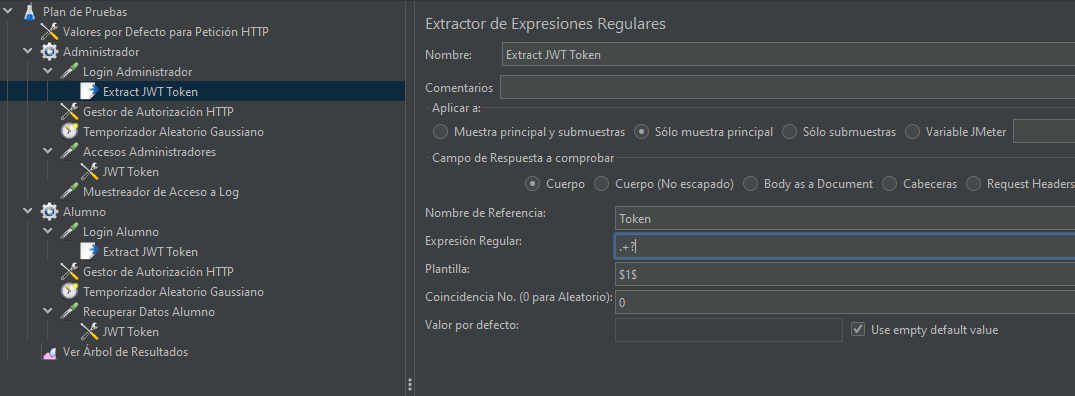
\includegraphics[width=\textwidth]{expresion regular config.png}
\end{figure}
\newline Y ahora configuramos los gestores de cabecera HTTP:
\newpage
\begin{figure}[hbt!]
    \centering
    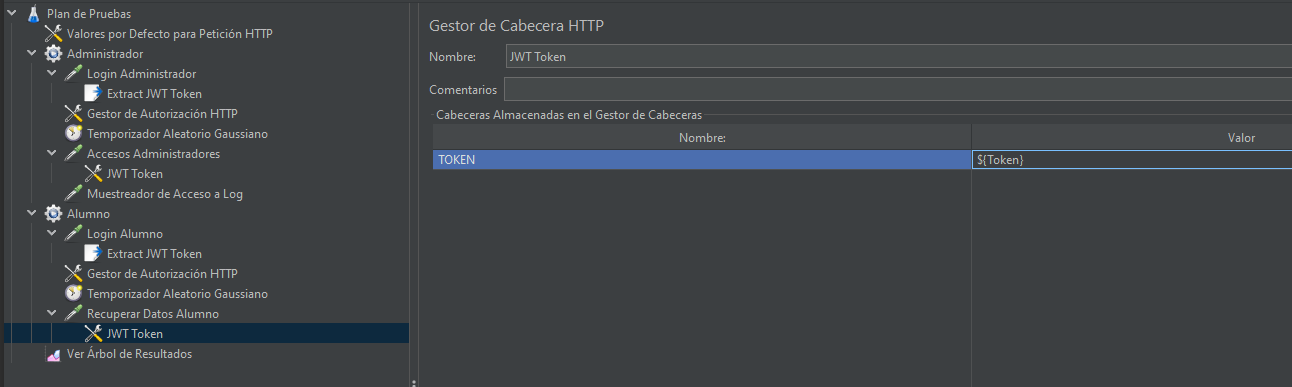
\includegraphics[width=\textwidth]{gestor cabecera config.png}
\end{figure}
\section{Ejercicio Opcional}
Con esta información usted podría modificar los parámetros
de configuración de Apache, PHP o MariaDB para observar un cambio en el
comportamiento del servidor (CentOS o Ubuntu server) mediante la aplicación
de un benchmark y analizando el cambio en las prestaciones o mediante el análisis
de datos de monitorización ante una carga aplicada.
\newpage
\begin{thebibliography}{99}
    \bibitem[Descargar Phoronix]{descargar phoronix} 
    \href{https://www.phoronix-test-suite.com/}{https://www.phoronix-test-suite.com/}
    \bibitem[Instalar Phoronix Ubuntu]{pagina ubuntuwiki para instalar phoronix}
    \href{https://wiki.ubuntu.com/PhoronixTestSuite#installing}{https://wiki.ubuntu.com/PhoronixTestSuite\#installing}
    \bibitem[OpenBenchmarking]{openbenchmarking} 
    \href{https://openbenchmarking.org/s}{https://openbenchmarking.org/s}
    \bibitem[Instalar Docker]{instalar docker} 
    \href{https://docs.docker.com/engine/install/}{https://docs.docker.com/engine/install/}
    \bibitem[Repositorio GitHub]{codigo github para Jmeter} 
    \href{https://github.com/davidPalomar-ugr/iseP4JMeter}{https://github.com/davidPalomar-ugr/iseP4JMeter}
    \bibitem[Apache JMeter]{pag oficial de jmeter} 
    \href{https://jmeter.apache.org/}{https://jmeter.apache.org/}
    \bibitem[Usar JMeter]{usermanual Jmeter}
    \href{https://jmeter.apache.org/usermanual/index.html}{https://jmeter.apache.org/usermanual/index.html}

\end{thebibliography}
\end{document}